\section{Model} \label{sec:model}

In this section, we describe the training data and the testing data provided by Kaggle, and introduce our model. 

\paragraph{Dataset}

The training data contains 4 fields: the tweet ID, the tweet, the selected tweet (supporting the sentiment), and the sentiment. The testing data contains 3 fields: the tweet ID, the tweet, and the sentiment. Samples of the training data, the testing data and our extracted supporting phrase are provided below.

\begin{table}[!h]
	\centering
	\begin{tabular} {c | l l c}
	Tweet ID & Tweet & Supporting phrase & Sentiment \\
	\hline
	af82 & headache wanna see my Julie & headache & negative \\
    09ca & Oh! Good idea baout putting them on ice cream & Good & positive \\
	1c2d & Thank a youu  how are you? & Thank & positive
	\end{tabular}
	\caption{Sample of training set}
\end{table} 

\begin{table}[!h]
	\centering
	\begin{tabular} {c | l c}
	Tweet ID & Tweet & Sentiment \\
	\hline
	a5be & i'm done. haha. HOUSE MD marachon ulet & positive \\
	bca1 & 26th Feb & neutral \\
	16ca & I wish I was calling you but i can't from Malta & positive 
	\end{tabular}
	\caption{Sample of testing set}
\end{table} 

\begin{table}[!h]
	\centering
	\begin{tabular} {c | l c}
	Tweet ID & Supporting phrase \\
	\hline
	a5be & haha \\
	bca1 & 26th Feb \\
	16ca & I wish I was calling 
	\end{tabular}
	\caption{Sample of predicted supporting phrase}
\end{table} 

The support phrases are extracted from \href{https://appen.com/resources/datasets/}{Figure Eight's Data for Everyone platform}. The dataset is titled Sentiment Analysis: Emotion in Text tweets with existing sentiment labels under the creative commons attribution 4.0. international licence. Our project is to essentially reproduce these supporting phrases.



\paragraph{Our model}

In this project, we assume that the supporting phrase is a contiguous substring of the tweet. Our model comprises a pre-trained BERT model (SPECIFICATIONS?) and a layer of linear regression on top of BERT, detailed below. 

Our use of the pre-trained BERT model can be viewed as a function $f_{bert}$ from the set of training tweets $T$ to $\mathbb{N}^{m \times d}$, where $m$ is a constant factor of the maximum number of tokens in a tweet and $d$ is some constant (due to BERT specifications): $$f_{bert}: T \rightarrow \mathbb{N}^{m \times d}.$$ It works as follows: We first tokenize and each tweet $t \in T$ and its supporting phrase $s_t$ into integer arrays $A_t$ and $A_{s_t}$, where the length of $A_t$ and $A_{s_t}$ are almost the same as the number of tokens in the tweet and the supporting phrase (due to BERT specifications). Then compute $i_{t}$ and $j_{t}$ such that $A_t[i_{t}, j_{t}] = A_{s_t}$, where $t[i,j]$ denote the subarray with index from $i$ to $j$ (both inclusive). We then collate all integer arrays $A_t$ into a vector  $x_t \in \mathbb{N}^{m}$, padding the short arrays with a padding token designated by BERT. We then feed all tweet vectors $x_t$ to a pre-trained BERT model, yielding output matrix $y_t$ of dimension $\mathbb{N}^{m \times d}$. We denote $y_t[i]$ as the $i$-th column vector of $y_t$.

Let $T^+$, $T^0$ and $T^-$ be the set of positive, neutral and negative training tweets respectively. We then apply a multinomial logistic regression to train weight vectors $w^{+,i}$, $w^{-,i}$, $w^{0,i}$, $w^{0,j}$, $w^{-,i}$, $w^{-,j} \in \mathbb{R}^d$, where $w^{s,i}$ and $w^{s, j}$ are trained on datasets $(y_{t}, i_t)$ for each $t \in T^s$ and $(y_{t}, j_t)$ for each $t \in T^s$ respectively.


Note that this training process not only modifies each weight vector $w^{s, i}$ and $w^{s, j}$, it modifies the parameters in BERT as well.


In the testing phase for each tweet $t$ with sentiment $s$, we compute first $y_t = f_{bert}(t)$ and then 
\begin{align*}
	i_{t} &= \arg\max_{k} (w^{s, i})^T y_t[k] \\
	j_{t} &= \arg\max_{k} (w^{s, j})^T y_t[k].
\end{align*}
Finally we report that the supporting phrase is the substring corresponding to the subarray $A_t[i_{t}, j_{t}]$. Note that if $i_{t} > j_{t}$, an empty string is returned.

 Figure~\ref{fig:model} illustrates the above process.

\begin{figure}[!h]
	\centering
	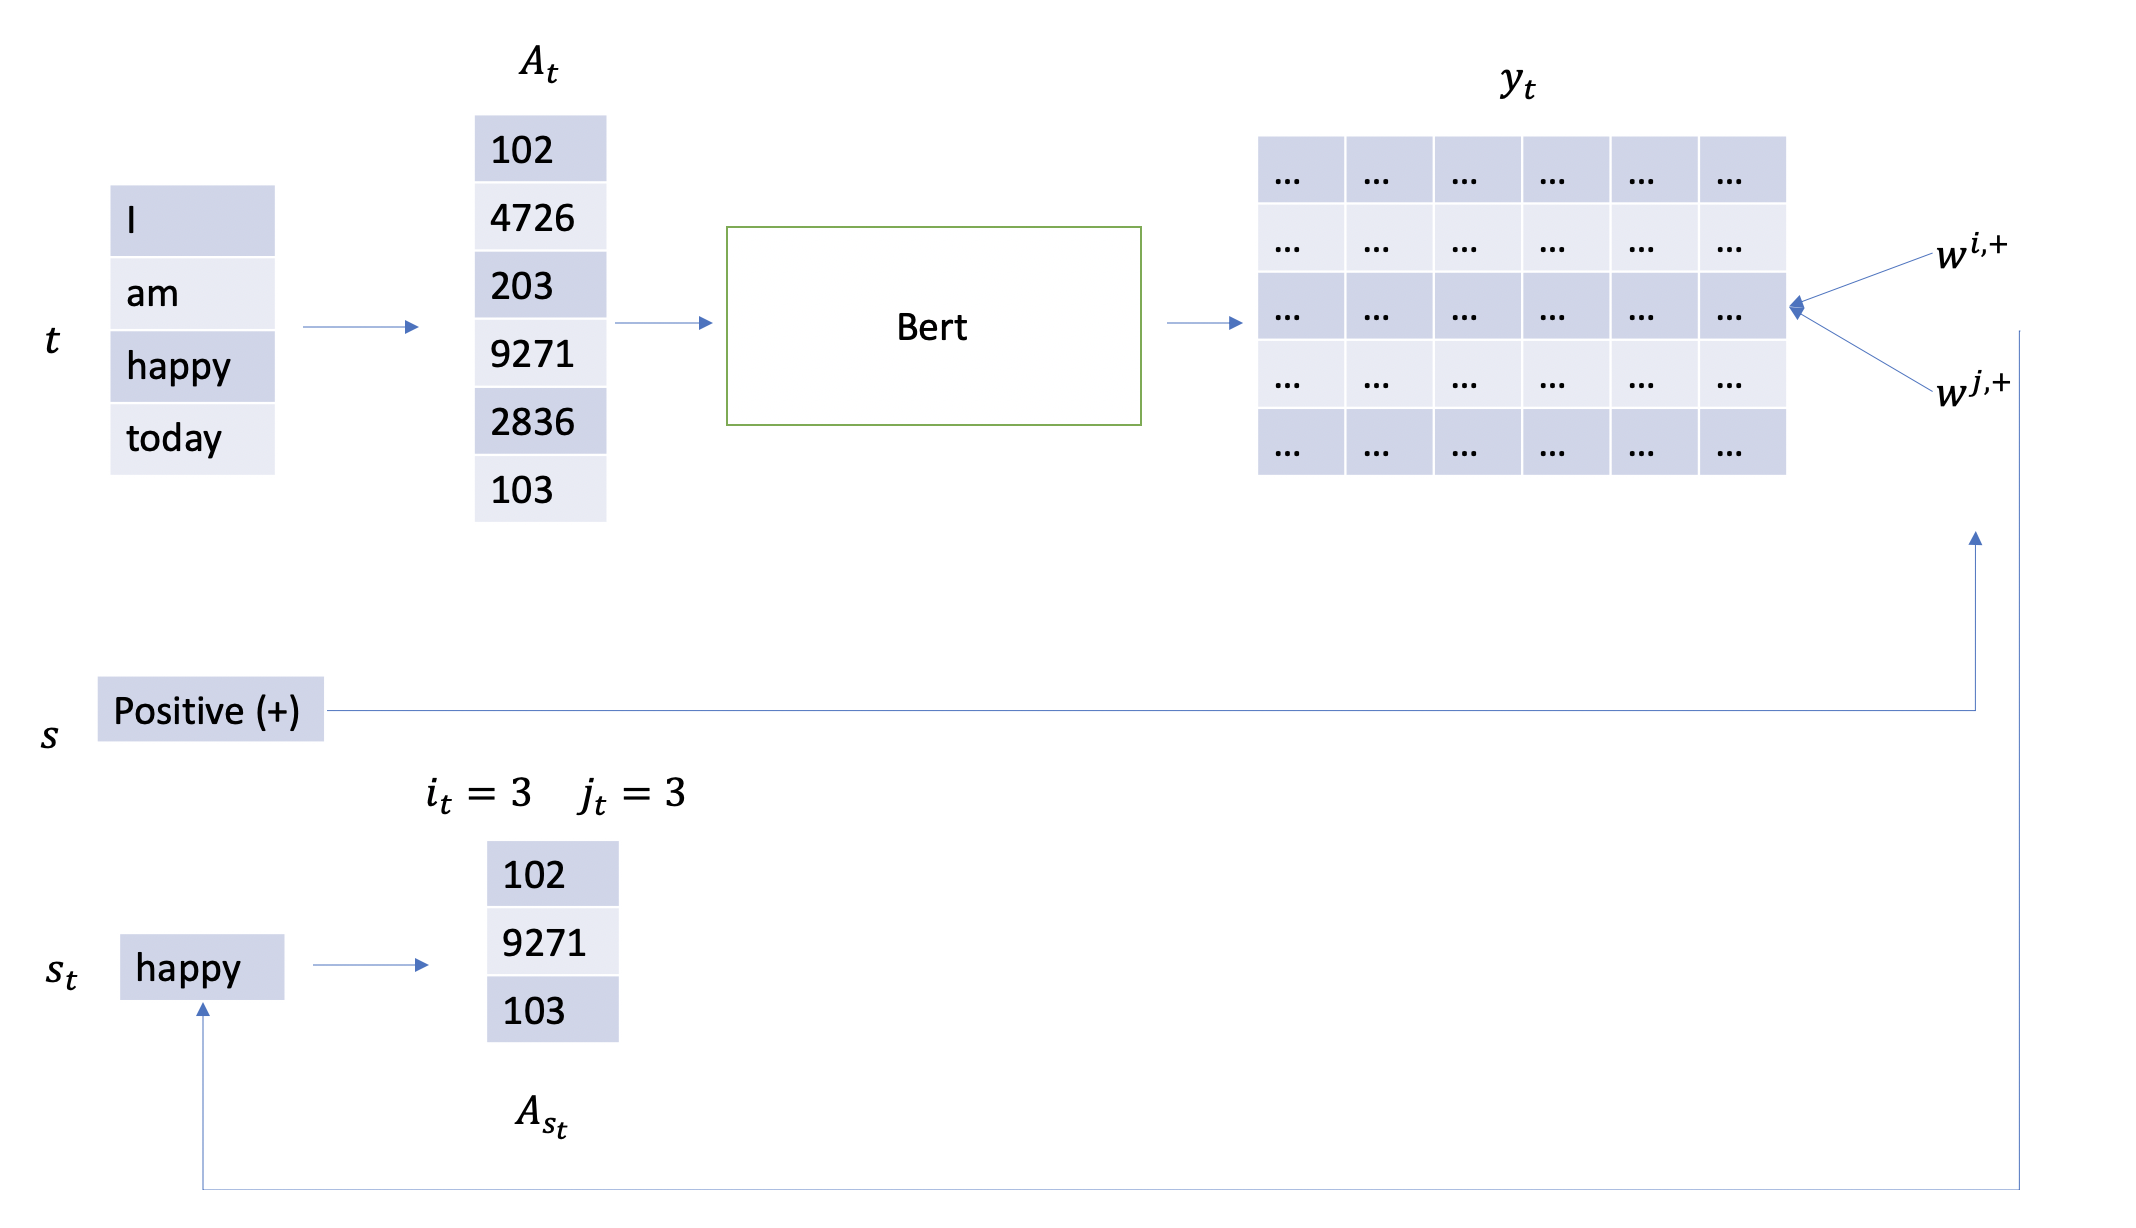
\includegraphics[width=0.7\textwidth,keepaspectratio]{model}
	\caption{Our model}
	\label{fig:model}
\end{figure}